%
% File naaclhlt2010.tex
%
% Contact: nasmith@cs.cmu.edu

\documentclass[11pt,letterpaper]{article}
\usepackage{naaclhlt2010}
\usepackage{times}
\usepackage{latexsym}
\usepackage{graphicx}
\usepackage{commath}

\setlength\titlebox{6.5cm}    % Expanding the titlebox

\title{Survey of Neighborhood-based Collaborative Filtering Techniques for a Movie Recommendation Engine}

\author{Nirmal Krishnan\\
  Johns Hopkins University\\
  9 E 33rd Street, 308 C\\
  Baltimore, MD 21218, USA\\
  {\tt nkrishn9@jhu.edu}
  \And
  Emily Brahma \\
  Johns Hopkins University \\
  9 E 33rd Street, 610 D \\
  Baltimore, MD 21218, USA\\
  {\tt ebrahma1@jhu.edu}}

\date{}

\begin{document}
\maketitle
\begin{abstract}
Collaborative filtering is a technique used for recommendation engines in which a user's interest in new items are computed based on the recommendations of users with similar interests. Almost all implementations of collaborative filtering use a neighbor-based prediction algorithm in which a subset of users that are similar to the active user are chosen. Based on this subset of users, predictions for new items for our active user (using a weighted average metric) are computed. However, there is no consensus on how to select this subset of users that are "similar" to our active user. In this study, we surveyed different similarity metrics for collaborative filtering in the context of movie ratings. When considering both few and many neighbors, cosine-similarity, one of the four similarity metrics surveyed, performed best (lowest mean absolute error). It is also the easiest to implement and runs efficiently using numpy optimizations. We recommend using cosine-similarity as the similarity metric for movie recommendation systems for these reasons.
\end{abstract}

\section{Introduction}
In 2009, Netflix offered a one million dollar prize to an individual that could create a recommendation engine better than its own. Many solutions were attempted, but the most successful algorithms were those that used a technique known as collaborative filtering, in which a user’s interest in new items are computed based on the recommendations of users with similar interests. Almost all implementations of collaborative filtering use a neighbor-based prediction algorithm similar to k-nearest neighbors (k-NN) (Herlocker et al. 2002). However, there is no consensus on how parameters are weighted, and what kind of similarity metrics are used. In this study, we will be surveying the effects of different parameter weighting techniques on neighborhood-based collaborative filtering in the context of the movie recommendation problem.


\section{Background}
\subsection{Vocabulary}
Since this paper involves a survey of algorithms found in the literature, it is important to first define some vocabulary in order to understand the structure of said algorithms.
\begin{itemize}
    \item \textbf{user:} a single person for who we have his or her past movie rating history
    \item \textbf{item:} a movie
    \item \textbf{rating:} a user's preference for a movie defined on a 0.5 to a 5 scale with 5 being the highest possible preference
    \item \textbf{intersection set:} for two users u and v, the intersection set consists of the movies both u and v have rated
    \item \textbf{active user:} the user for whom we are predicting a rating for a movie the user has not seen/rated
\end{itemize}
\subsection{What is Collaborative Filtering?}
Collaborative filtering, as defined by Extstrand et al, "is a recommendation algorithm that bases its predictions and recommendations on the ratings or behavior of other users in the system." This approach is based on the assumption that users with similar tastes will rate the same item similarly. Consequently, most collaborative filtering techniques employ a neighbor-based approach in order to determine a set of users that are similar to our active user. Neighbor based algorithms generally consist of finding the k-closest training examples in the feature space (Altman et al).
Consider the example below:
\begin{center}
 \begin{tabular}{||c c c c||}
 \hline
  & Superman & Up & The Incredibles \\ [0.5ex]
 \hline\hline
 User 1 & 5 & 1 & 5 \\
 \hline
 User 2 & 5 & 1 & ? \\
 \hline
 User 3 & 2 & 5 & 3 \\
 \hline
 User 4 & 3 & ? & 3 \\
 \hline
 User 5 & 3 & 5 & 2 \\
 \hline
\end{tabular}
\end{center}
Let us first consider User 2 to be the active user (since we do not have a rating for The Incredibles). A good collaborative filtering technique would see that User 1 and User 2 rated Superman and Up exactly the same way, but User 2 and Users 3, 4, and 5 have little similarity in their rating tendencies. Therefore, User 1's movie recommendation history would be most heavily considered and our collaborative filtering technique would potentially rate The Incredibles for User 2 as a 5.\\
Let us now consider User 4 as our active user (since we do not have a rating for Up). User 4, 3, and 5 were apathetic towards Superman and the Incredibles, while Users 1 and 2 highly preferred Superman and the Incredibles. Consequently, a good collaborative filtering algorithm would weight the preferences of Users 3 and 5 more than that of 1 and 2, giving a predicted rating of Up for User 4 to be 5.\\
This type of collaborative filtering where we find users similar to our active user is known as user-user collaborative filtering.\\
Unlike in user-user collaborative filtering, item-item collaborative filtering uses the similarities of items to make recommendations. As described by Extstrand et al, Item-item collaborative filtering "uses similarities between the rating patterns of items. If two items tend to have the same users like and dislike them, then they are similar and users are expected to have similar preferences for similar items."\\
This study, however, focuses only on user-user collaborative filtering.

\section{Methods}
In terms of programming tools, we used Python to build our movie recommendation engine. We also used numpy and Python's collections library to structure the data efficiently. The data that we used for the study is publicly available through an online database called MovieLens. This database contains 100,004 ratings created by 671 users, and covers 9,125 movies. Each user was chosen at random and has rated at least 20 movies, ensuring that the data-set is not too sparse for analysis. Our move recommendation engine's general approach is  as follows:
\begin{enumerate}
    \item Pick an active user for which we would like to predict that user’s rating for an arbitrary movie.
    \item Use a weighting technique to weigh all of the users in the data-set for similarity to the active user.
    \item Pick a set of users based on closest similarity to active user.
    \item Make a prediction based on the subset selected in part 3
\end{enumerate}
In terms of picking what user and movie to make a prediction for (step 1), we make rating predictions for all the users in the data one at a time, in the order in which they appear. For each user, we include every movie the active user has rated except the active user’s 10th to 20th movie rating for computing the similarity between the active user and all other users. The active user’s 10th to 20th movies are the movies we will actually make a prediction on.
\\ \\In step 2, we explore four different similarity wighting schemes: (1) Pearson Correlation Coefficient, (2) Spearman Rank Correlation Coefficient, (3) Mean-Squared Distance, and (4) Cosine Similarity. We can observe how different weighting schemes affect which users are considered to be "similar" and which are not.
\\ \\The number of users that are to be chosen in step 3 is $k$, a parameter passed in at the start of the program. Thus, it is the $k$ users that have the highest similarity value in relation to the active user that are picked in this step.
\\ \\Once we have the $k$ most similar users to the active users, we make our rating prediction for movie $i$ (Step 4) based on a weighted average defined as follows:
$$\hat{y} = \bar{r_u} + \frac{\sum_{v\in N}s(u,v)(r_{v,i} - \bar{r_{v}})}{\sum_{v\in N}|s(u,v)|}$$
\\such that
\begin{itemize}
\item $u$ - active user
\item $v$ - any other user
\item N - set of $k$ most similar users to $u$
\item $r_{v,i}$ - user $v$'s rating of movie $i$
\item $\bar{r}$ - user's average movie rating
\item $s(u,v)$ - similarity between active user $u$ and user $v$
\end{itemize}

\subsection{Evaluation:}
We used the mean absolute error to measure the error of the ratings produces by each similarity weighting metric. The mean absolute error is defined to be just as it sounds where:
$$MAE = \frac{1}{n}\sum_{i = 1}^n|\hat{y_i} - y_i|$$
$\hat{y_i}$ is the predicted rating for movie $i$ and $y_i$ is the real rating.

\section{Implementation}
\subsection{Pearson Correlation Coefficient}
The Pearson Correlation Coefficient takes the intersection ($I_{u} \cap I_{v}$) of the movies rated by the active user $u$ and every other user $v$  and computes the statistical correlation of the ratings between the two users in this set. The similarity between user $u$ and $v$ is defined by the Pearson Correlation Coefficient as follows:\\\\
$s(u,v) = \frac{\sum_{i \in I_{u} \cap I_{v}} (r_{u, i} - \bar r_{u}) (r_{v, i} - \bar r_{v})}{\sqrt{\sum_{i \in I_{u} \cap I_{v}}(r_{u, i} - \bar r_{u})^2} \sqrt{\sum_{i \in I_{u} \cap I_{v}}(r_{v, i} - \bar r_{v})^2}} $\\

\subsection{Spearman Rank Correlation Coefficient}
The Spearman Rank Correlaton Coefficient computes similarity between two users similarly to the Pearson approach. However, the Spearman weighting scheme considers the rank that a movie takes on instead of its rating. As described by Ekstrand et al, "items a user has rated are ranked such that their highest-rated item is at rank 1 and lower- rated items have higher ranks. Items with the same rating are assigned the average rank for their position." The Spearman Correlation defines the similarity between user $u$ and $v$ as follows:\\\\
$s(u,v) = \frac{\sum_{i \in I_{u} \cap I_{v}} (k_{u, i} - \bar k_{u}) (k_{v, i} - \bar k_{v})}{\sqrt{\sum_{i \in I_{u} \cap I_{v}}(k_{u, i} - \bar k_{u})^2 \sum_{i \in I_{u} \cap I_{v}}(k_{v, i} - \bar k_{v})^2}} $\\
\\Here, $k_{u,i}$ represents movie $i$'s \textit{ranking} amongst user $u$'s ratings. As we can see, the Spearman Rank Correlation Coefficient is the same as the Pearson Correlation defined before, but with ratings swapped out for rankings.
\subsection{Mean-Squared Distance}
The mean-squared distance similarity scheme is essentially just as it sounds. We sum the squared difference between user $u$ and user $v$'s ratings over their common movies and divide by the number of common movies. This metric emphasizes penalizing difference in tastes over rewarding similarity in taste. The mean-squared distance scheme is defined as:
$$s(u,v) = \frac{\sum_{i \in I_{u} \cap I_{v}} (r_{u, i} - r_{v,i})^2}{|I_{u} \cap I_{v}|}$$
\subsection{Cosine Similarity}
The cosine similarity metric takes a different approach to finding the similarity between users, unlike the statistical approaches we've described before. With cosine similarity, each user is considered as a vector of his or her ratings, so that the similarity metric is essentially the cosine distance between these to vectors. The cosine similarity metric is defined as:
$$s(u,v) = \frac{r_u \cdot r_v}{\norm{r_u}\norm{r_v}}$$
\\where $r_u$ and $r_v$ are the ratings vectors for movies rated by both users $u$ and $v$.
\section{Results}
In the literature, most studies have concluded that Pearson Correlation Coefficient will perform the best of the four similarity metrics we surveyed. Herlocker et al concluded that "For those who are considering using a neighborhood-based prediction algorithm to perform automated collaborative filtering, we have the following recommendations: Use Pearson correlation as a similarity measure: it remains the most accurate technique for computing similarity." This conclusion was drawn when 60 neighbors were considered. \\
In our study, we initially ran our four similarity metrics using 10 neighbors to all neighbors (in 10-neighbor increments). The results can be found below.
\begin{figure}[h]
\caption{Comparison of Similarity Techniques from 10 Neighbors to All Neighbors}
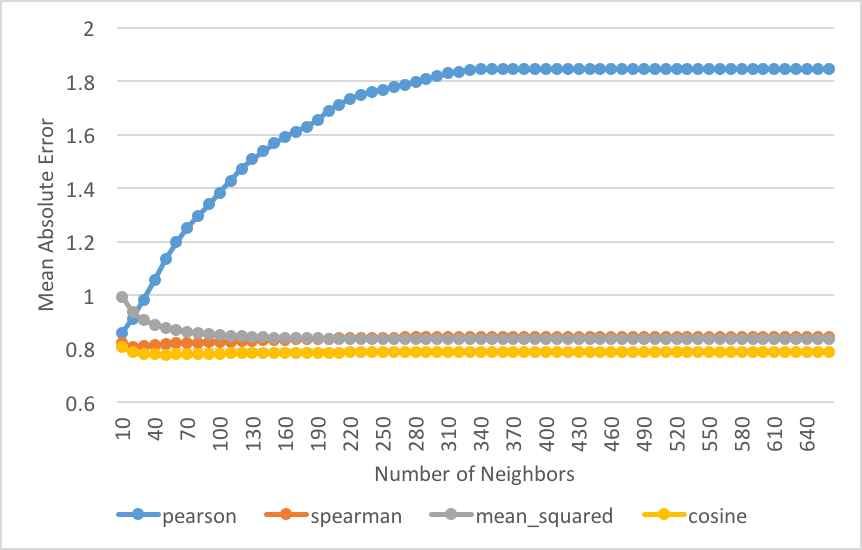
\includegraphics[scale = 0.55]{graph1.png}
\centering
\end{figure}
\\
From Figure 1, it appears Pearson Correlation Coefficient performs poorly as the number of neighbors considered increases. It appears to flatline at approximately 310 neighbors (half off the dataset) when the mean absolute error is approximately 1.8. This is an extremely poor result for Pearson Correlation Coefficient because a mean absolute error of ~2 indicates that our recommendation system is generally wrong (a prediction of 4 may actually be a 2, a prediction of 1 may actually be a 3, etc.). Therefore, it appears using Pearson Correlation Coefficient with a large set of neighbors is not recommended. \\
The other three filtering techniques seem to perform similarly, and actually improve in accuracy as the number of neighbors considered increases. Between these three techniques, Mean-Squared Distance appears to perform the worst when the number of neighbors considered is few. Spearman Rank Correlation Coefficient and Cosine Similarity perform similarly, with the latter edging Spearman Rank Correlation Coefficient in accuracy slightly when the number of neighbors considered is few. However, as the number of neighbors considered increases, Cosine Similarity flatlines at approximately .78 MAE, while Spearman Rank Correlation Coefficient and Mean-Square Distance flatline at .84 MAE. Therefore, Cosine Similarity seems to be the optimal approach when the number of neighbors considered is greater than 10. Figure 2 shows the results when the number of neighbors considered is less than 10.

\begin{figure}[h]
\caption{Comparison of Similarity Techniques from 2 Neighbors to 10 Neighbors}
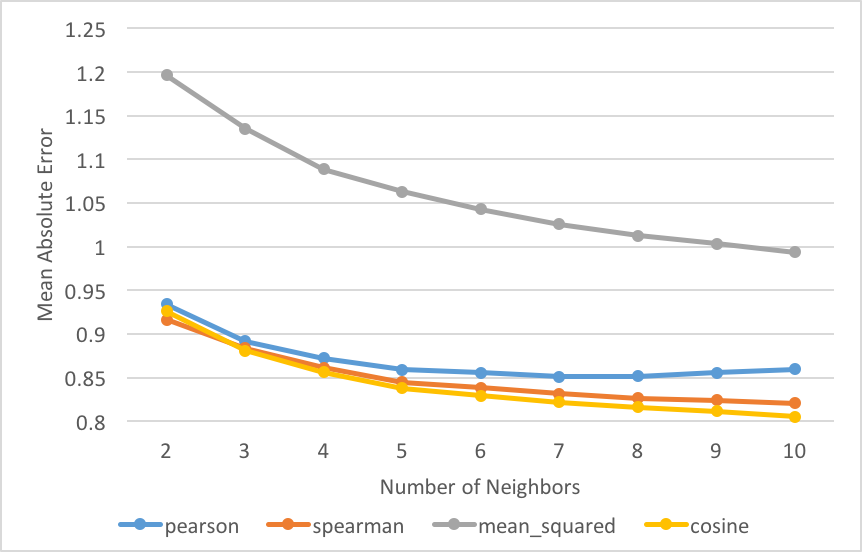
\includegraphics[scale = 0.55]{graph2.png}
\centering
\end{figure}


From figure 2, we can see that Pearson Correlation Coefficient operates significantly better when the number of neighbors considered is few. It appears it reaches its optimal point of MAE at 7 neighbors, with MAE increasing after this point. Mean-squared Distance performs poorly when the number of neighbors is less than 10 with a consistent MAE of greater than 1. Spearman Rank Correlation Coefficient and Cosine Similarity perform almost identically again, with Cosine Similarity again edging Spearman Rank Correlation Coefficient in accuracy as the number of neighbors considered increases. Therefore, for both small and large number of neighbors considered, Cosine Similarity performs the best (minimal MAE) of our four similarity metrics. In terms of speed as well, Cosine-Similarity performs well because of Numpy optimizations that allow dot product and Euclidean norm's to be calculated quickly and efficiently. Consequently, for a movie recommendation engine, we recommend using Cosine-Similarity over the other three techniques described.

\section{Analysis of Results:}
In our results, Pearson Correlation Coefficient performs poorly across the board of number of neighbors considered (compared to the other algorithms). We propose this is the case due to this metric's tendency to compute a high similarity for users with few items in common. Consider the example below:
\begin{center}
 \begin{tabular}{||c c c||}
 \hline
  & The Fugitive & Up \\ [0.5ex]
 \hline\hline
 User u & 5 & 1  \\
 \hline
 User v & 5 & 1  \\
 \hline
\end{tabular}
\end{center}
User's 1 and 2 only have only rated two movies in common: the Fugitive and Up. All other movies watched by the two users are distinct and do not appear in the intersection set $I_{u} \cap I_{v}$.
Therefore, the Pearson Correlation Coefficient will compute similarity between the users u and v as follows:
$s(u,v) = \frac{\sum_{i \in I_{u} \cap I_{v}} (r_{u, i} - \bar r_{u}) (r_{v, i} - \bar r_{v})}{\sqrt{\sum_{i \in I_{u} \cap I_{v}}(r_{u, i} - \bar r_{u})^2} \sqrt{\sum_{i \in I_{u} \cap I_{v}}(r_{v, i} - \bar r_{v})^2}} $\\
$s(u,v) = \frac{(1-3)(1-3)+ (5-3)(5-3)}{\sqrt{(1-3)^2 + (5-3)^2} \sqrt{(1-3)^2 + (5-3)^2}}$ \\
$s(u,v) = \frac{8}{8} = 1$\\
Based on this computation, the similarity between these two users, u and v, is 1, meaning the users are a perfect match (identically similar). However, the two users have only rated two movies in common, so it is possible that these two movies were an aberration: the user's do not actually have the same tastes in movies. However, since Pearson Correlation Coefficient does not have a way of correcting for users having few ratings in common, this type of miscomputation of similarity may be common in real usage. Ekstrand et al recommends "setting a threshold on the number of co-rated items necessary for full agreement (correlation of 1) and scaling the similarity when the number of co-rated items falls below this threshold." This may lead to better results and through empirical testing, it appears this is the case. However, there is little consensus on what threshold is optimal, so we recommend more studies be performed on this threshold-based Pearson Correlation Coefficient. \\
In regards to the other three algorithms, the differences between them are not statistically significant (using a p-value of 0.05). However, we are recommending Cosine-Similarity for the following reasons:
\begin{itemize}
\setlength\itemsep{0em}
    \item mean absolute error is consistently below 0.8
    \item easy to implement and test
    \item numpy optimizations allow this to operate efficiently and quickly on large datasets
\end{itemize}


\section{Comparison to Proposal}
In our proposal for this project, we listed the following goals:
\subsection{Must achieve}
We must achieve an implementation of collaborative filtering that uses all three of the weighting similarity techniques listed above, such that we can make a recommendation on the best one.
\subsection{Expected to achieve}
We are expected to achieve an implementation of a non-statistical technique for collaborative filtering. This approach, known as cosine similarity, is based on a linear algebra design where users are treated as $|N|$-dimensional vectors and "similarity is measured
by the cosine distance between two rating vectors." We would like see how this technique compares with the traditional statistical approaches.
\subsection{Would like to achieve}
If possible, we would like to survey other weighting similarity techniques that could potentially yield better results. These techniques may include Constrained Pearson correlation and Pearson Correlation with threshold-based damping. If time permits, we would also like to brainstorm and test ideas for our own similarity metric.
\subsection{What we actually achieved}
We achieved the goals listed in both 6.1 and 6.2 in that we wrote an implementation for four different similarity metrics for Collaborative Filtering. We did not achieve section 6.3 in strict terms, however, we did perform a comparative analysis of these algorithms on different number of neighbor parameters. We felt that it was important to show how these algorithms performed under different parameters and this analysis allowed us to make an informed recommendation on which algorithm to choose when number of neighbors considered is small and when it is large.


\begin{thebibliography}{}

\bibitem[\protect\citename{Herlocker, Konstan, and Riedl}2002]{Herlocker}
Herlocker, Konstan, and Riedl.
\newblock 2002.
\newblock {\em An Empirical Analysis of Design Choices in Neighborhood-Based Collaborative Filtering Algorithms.}, Information Retrieval, 5.


\bibitem[\protect\citename{{Ekstrand, Riedl, and Konstan}}2011]{Ekstrand}
{Ekstrand, Riedl, and Konstan}.
\newblock 2011.
\newblock {\em Collaborative Filtering Recommender Systems}.
\newblock Foundations and Trends in Human–Computer Interaction. Vol. 4, No. 2.

\bibitem[\protect\citename{{Melville, Mooney, and Nagarajan}}2002]{Melville}
{Melville, Mooney, and Nagarajan}.
\newblock 2002.
\newblock {\em Content-Boosted Collaborative Filtering for Improved Recommendations}.
\newblock Proceedings of the Eighteenth National Conference on Artificial Intelligence, Edmonton, Canada.

\bibitem[\protect\citename{Breese, Heckerman, and Kadie}1998]{Breese}
Breese, Heckerman, and Kadie.
\newblock 1998.
\newblock {\em Empirical analysis of predictive algorithms for collaborative filtering.}

\bibitem[\protect\citename{Cooper and Moral}1998]{Cooper and Moral}
Cooper and Moral
\newblock 1998.
\newblock {\em Empirical analysis of predictive algorithms for collaborative filtering}.
\newblock Proceedings of the Fourteenth Conference on Uncertainty in Artificial Intelligence. San Francisco.

\end{thebibliography}

\end{document}
